\documentclass{beamer}

\newcommand{\course}{CS 1331 Introduction to Object Oriented Programming}
\newcommand{\lesson}{Data Abstraction}
\newcommand{\code}{http://www.cc.gatech.edu/~simpkins/teaching/gatech/cs1331/code}

\author[Chris Simpkins]
{Christopher Simpkins \\\texttt{chris.simpkins@gatech.edu}}
\institute[Georgia Tech] % (optional, but mostly needed)

\date{}


\newcommand{\course}{Introduction to Object-Oriented Programming}
\subject{\course}
\title[\lesson]{\course}
\subtitle{\lesson}

\author[CS 1331]
{Christopher Simpkins \\\texttt{chris.simpkins@gatech.edu}}
\institute[Georgia Tech]

\date[]{}

\newcommand{\link}[2]{\href{#1}{\textcolor{blue}{\underline{#2}}}}
\newcommand{\code}{http://www.cc.gatech.edu/~simpkins/teaching/gatech/cs1331/code}

\usepackage{colortbl}

% If you have a file called "university-logo-filename.xxx", where xxx
% is a graphic format that can be processed by latex or pdflatex,
% resp., then you can add a logo as follows:

% \pgfdeclareimage[width=0.6in]{coc-logo}{cc_2012_logo}
% \logo{\pgfuseimage{coc-logo}}

\mode<presentation>
{
  \usetheme{Berlin}
  \useoutertheme{infolines}

  % or ...

 \setbeamercovered{transparent}
  % or whatever (possibly just delete it)
}

\usepackage{tikz}
% Optional PGF libraries
\usepackage{pgflibraryarrows}
\usepackage{pgflibrarysnakes}
\usepackage{pgfplots}
\usepackage{fancybox}
\usepackage{listings}
\usepackage[abbr]{harvard}
\usepackage{hyperref}
\hypersetup{colorlinks=true,urlcolor=blue}
\usepackage[english]{babel}
% or whatever

\usepackage[latin1]{inputenc}
% or whatever

\usepackage{times}
\usepackage[T1]{fontenc}
% Or whatever. Note that the encoding and the font should match. If T1
% does not look nice, try deleting the line with the fontenc.


\usepackage{listings}

% "define" Scala
\lstdefinelanguage{scala}{
  morekeywords={abstract,case,catch,class,def,%
    do,else,extends,false,final,finally,%
    for,if,implicit,import,match,mixin,%
    new,null,object,override,package,%
    private,protected,requires,return,sealed,%
    super,this,throw,trait,true,try,%
    type,val,var,while,with,yield},
  otherkeywords={=>,<-,<\%,<:,>:,\#,@},
  sensitive=true,
  morecomment=[l]{//},
  morecomment=[n]{/*}{*/},
  morestring=[b]",
  morestring=[b]',
  morestring=[b]""",
}

\usepackage{color}
\definecolor{dkgreen}{rgb}{0,0.6,0}
\definecolor{gray}{rgb}{0.5,0.5,0.5}
\definecolor{mauve}{rgb}{0.58,0,0.82}

% Default settings for code listings
\lstset{frame=tb,
  language=scala,
  aboveskip=2mm,
  belowskip=2mm,
  showstringspaces=false,
  columns=flexible,
  basicstyle={\scriptsize\ttfamily},
  numbers=none,
  numberstyle=\tiny\color{gray},
  keywordstyle=\color{blue},
  commentstyle=\color{dkgreen},
  stringstyle=\color{mauve},
  frame=single,
  breaklines=true,
  breakatwhitespace=true,
  keepspaces=true
  %tabsize=3
}


% \beamerdefaultoverlayspecification{<+->}


\begin{document}

\begin{frame}
  \titlepage
\end{frame}


%------------------------------------------------------------------------
\begin{frame}{Data Abstraction}


An abstraction of a concept attempts to capture the essence of the concept -- its essential properties and behaviors -- by ignoring irrelevant details.
\begin{itemize}
\item Process abstraction - group the operations of a process in a subprogram and expose only the essential elements of the process to clients through the subprogram signature (e.g., function/method name and parameters)
\item Data abstraction - encapsulation of data with the operations defined on the data
\item A particular data abstraction is called an {\em abstract data type}.  Note that ADT's include process abstractions as well
\end{itemize}

In each case, an abstraction hides details --- details of a process or details of a data structure.

\begin{quote}
``Abstraction is selective ignorance.''\\
-- Andrew Koenig (C++ Guru)
\end{quote}
\end{frame}
%------------------------------------------------------------------------

%------------------------------------------------------------------------
\begin{frame}[fragile]{A Complex Number ADT}


{\bf ADT: Complex}\\
Data:
\begin{itemize}
\item {\bf real: double} the real part of a complex number
\item {\bf imaginary: double} the imaginary part of a complex number
\end{itemize}
Operations:
\begin{itemize}
\item {\bf new} - construct a new complex number
\item {\bf plus} - add one complex number to another, yielding a new complex number
\end{itemize}
An ADT is {\it abstract} because the data and operations of the ADT are defined independently of how they are implemented.  We say that an ADT {\it encapsulates} the data and the operations on the data.

\end{frame}
%------------------------------------------------------------------------

%------------------------------------------------------------------------
\begin{frame}{Data Abstractions with Classes}

Java provides langauge suppport for defining ADTs in the form of classes.\\

A class is a blueprint for objects.  A class definition contains
\begin{itemize}
\item instance variables, a.k.a. member variables or fields -- the state, or data of an object
\item methods, a.k.a. member functions or messages -- the operations defined on objects of the class
\end{itemize}
We {\em instantiate} or {\em construct} an object from a class.
\end{frame}
%------------------------------------------------------------------------


%------------------------------------------------------------------------
\begin{frame}[fragile]{Java Implementation of Complex Number ADT}\label{complex-class}


Here's a Java implementation of our complex number ADT \footnote{\url{http://introcs.cs.princeton.edu/java/33design/}}:
\vspace{-.05in}
\begin{lstlisting}[language=Java]
public class Complex {
    // These are the data of the ADT

    private double real;
    private double imaginary;

    // These are the operations of the ADT

    public Complex(double aReal, double anImaginary) {
        real = aReal;
        imaginary = anImaginary;
    }

    public Complex plus(Complex other) {
        double resultReal = this.real + other.real;
        double resultImaginary = this.imaginary + other.imaginary;
        return new Complex(resultReal, resultImaginary);
    }
}
\end{lstlisting}


\end{frame}
%------------------------------------------------------------------------

%------------------------------------------------------------------------
\begin{frame}[fragile]{Reference Variables}


Consider the following code:
\begin{lstlisting}[language=Java]
Complex a = new Complex(1.0, 2.0);
Complex b = new Complex(3.0, 4.0);
Complex c = a.plus(b);
\end{lstlisting}

{\tt a}, {\tt b}, and {\tt c} are {\it reference} variables of type {\tt Complex}.  Reference variables have one of two values:

\begin{itemize}
\item the address of an object in memory (in this case an instance of {\tt Complex}), or
\item {\tt null}, meaning the variable references nothing.
\end{itemize}

\end{frame}
%------------------------------------------------------------------------

%------------------------------------------------------------------------
\begin{frame}[fragile]{Invoking Constructors}


The line:
\begin{lstlisting}[language=Java]
Complex a = new Complex(1.0, 2.0);
\end{lstlisting}

invokes the {\tt Complex} constructor, passing arguments {\tt 1.0} and {\tt 2.0}:

\begin{lstlisting}[language=Java,escapechar=`]
public Complex(aReal=`\colorbox{yellow}{1.0}`, anImaginary=`\colorbox{yellow}{2.0}`) {
    real = `\colorbox{yellow}{1.0}`;
    imaginary = `\colorbox{yellow}{2.0}`;
}
\end{lstlisting}

which {\it instantiates} a {\tt Complex} object and stores its address in the variable {\tt a}:

\begin{lstlisting}[language=Java]
Complex a = new Complex(1.0, 2.0);
\end{lstlisting}
Constructors initialize objects.  After the line above, {\tt Complex} object {\tt a}'s instance variables have the values {\tt 1.0} and {\tt 2.0}.

\end{frame}
%------------------------------------------------------------------------

%------------------------------------------------------------------------
\begin{frame}[fragile]{Visualizing Objects and Instantiation}

The object creation expression {\tt new Complex(1.0, 2.0)}
%% \begin{lstlisting}[language=Java]
%% new Complex(1.0, 2.0)
%% \end{lstlisting}
applies the {\tt Complex} blueprint defined by the class definition from slide \ref{complex-class}:
\vspace{-.1in}
\begin{center}
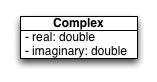
\includegraphics[height=.7in]{complex-class.png}
\end{center}
\vspace{-.125in}
to the constructor arguments {\tt (1.0, 2.0)} to create an instance of {\tt Complex}:
\vspace{-.125in}
\begin{center}
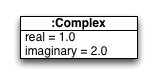
\includegraphics[height=.7in]{complex-instance.png}
\end{center}
\vspace{-.125in}
We can assign this object to a reference variable, e.g.,\\ {\tt Complex a = new Complex(1.0, 2.0)}:
%% \begin{lstlisting}[language=Java]
%% Complex a = new Complex(1.0, 2.0);
%% \end{lstlisting}
\vspace{-.075in}
\begin{center}
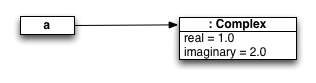
\includegraphics[height=.7in]{complex-reference.png}
\end{center}

\end{frame}
%------------------------------------------------------------------------


%------------------------------------------------------------------------
\begin{frame}[fragile]{Invoking Methods on Objects}


The line:
\begin{lstlisting}[language=Java]
Complex c = a.plus(b);
\end{lstlisting}
invokes the {\tt plus} method on the {\tt a} object, passing the {\tt b} object as an argument, which binds the object referenced by {\tt b} to the parameter {\tt other}:
\begin{lstlisting}[language=Java,escapechar=`]
a.plus(other=`\colorbox{yellow}{b}`) {
  double resultReal = this.real + `\colorbox{yellow}{b}`.real; // 1.0 + 3.0
  double resultImaginary = this.imaginary + `\colorbox{yellow}{b}`.imaginary; // 2.0 + 4.0
  return new Complex(resultReal, resultImaginary);
}
\end{lstlisting}
which returns a new {\tt Complex} object and assigns its address to the  reference variable {\tt c}.

\end{frame}
%------------------------------------------------------------------------

%------------------------------------------------------------------------
\begin{frame}[fragile]{Using the {\tt Complex} Class}


Users, or {\it clients} of the {\tt Complex} class can then write code like this:
\begin{lstlisting}[language=Java]
Complex a = new Complex(1.0, 2.0);
Complex b = new Complex(3.0, 4.0);
Complex c = a.plus(b);
\end{lstlisting}

without being concerned with {\tt Complex}'s implementation (which could use polar form, for example).  Clients (i.e., users) of the {\tt Complex} class need only be concerned with its interface, or {\it API} (application programmer interface) -- the public methods of the class.\\
\vspace{.1in}
After the code above we have the following {\tt Complex} objects in memory:
\begin{center}
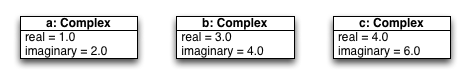
\includegraphics[height=.7in]{complex-abc.png}
\end{center}

\end{frame}
%------------------------------------------------------------------------



% %------------------------------------------------------------------------
% \begin{frame}[fragile]{}


% \begin{lstlisting}[language=Java]

% \end{lstlisting}

% \begin{itemize}
% \item
% \end{itemize}


% \end{frame}
% %------------------------------------------------------------------------


\end{document}
